\documentclass[journal]{IEEEtran}
\usepackage{amsmath,amssymb,amsthm}
\usepackage{hyperref}
\usepackage{booktabs}
\usepackage{graphicx}
\usepackage{algorithm}
\usepackage{algpseudocode}
\usepackage{xcolor}
\usepackage{cite}

% ─── Theorem environments ─────────────────────────────────────────────────────
\newtheorem{theorem}{Theorem}
\newtheorem{lemma}{Lemma}
\newtheorem{corollary}{Corollary}
\newtheorem{definition}{Definition}
\newtheorem{proposition}{Proposition}

\title{Towards an AI-Native Blockchain Framework:\\
Integrating Proof of Useful Intelligence, Zero-Knowledge\\
Machine Learning Security, and Post-Quantum Cryptography}

\author{Md. Mehedi Hasan, Asraful Islam Sharthak, \\
and Prof. Dr. Md. Abdul Based,~\IEEEmembership{Principal Investigator}
\IEEEcompsocitemizethanks{
  \IEEEcompsocthanksitem Manuscript submitted to IEEE Transactions on Dependable
  and Secure Computing (TDSC). \hfil\break
  \IEEEcompsocthanksitem Corresponding author: Md. Mehedi Hasan.
}}

\begin{document}
\maketitle

%─────────────────────────────────────────────────────────────────────────────
\begin{abstract}
Traditional blockchain consensus mechanisms face a series of critical bottlenecks. Existing Proof-of-Work and Proof-of-Stake protocols secure distributed networks but expend massive computational and capital resources without advancing scientific or artificial intelligence (AI) research. Concurrently, emerging solutions that utilize Zero-Knowledge Machine Learning (ZKML) to verify AI inferences suffer from formally undercharacterized vulnerability classes. These flaws allow malicious validators to forge proofs and compromise the network's integrity. Furthermore, the inevitable transition to post-quantum cryptography (PQC) introduces significant measurement overheads that remain largely unquantified within AI-intensive consensus environments. In this paper, we address these interconnected challenges by proposing a comprehensive, co-designed framework. First, we introduce and formally prove a Trust Score model for a Proof of Useful Intelligence (PoUI) consensus mechanism. Our formal analysis establishes strict bounds on trust scores, guarantees Sybil resistance, ensures non-gameability under rational adversarial assumptions, and provides convergence theorems for the rapid exclusion of malicious nodes. Extensive simulations ($N=100$ nodes over $1{,}000$ epochs) demonstrate a 100\% malicious exclusion rate. Second, we present the first formal taxonomy of underconstrained ZKML circuit vulnerabilities tailored to blockchain validators, outlining five specific attack classes and necessary constraint conditions to ensure circuit soundness. Third, we benchmark the overhead of ML-DSA and ML-KEM post-quantum cryptographic standards at scale, revealing that ML-DSA-44 is highly feasible across various throughput targets when coupled with appropriate block-size mitigations. Finally, we formally define the interface contracts that govern the integration of PoUI, ZKML, and PQC, highlighting emergent security properties and previously unexposed failure modes specific to their co-design. This work ultimately delivers a unified, formally grounded architectural blueprint for building AI-native blockchains that are resilient against both classical and quantum adversaries.
\end{abstract}

\begin{IEEEkeywords}
Proof of Useful Intelligence, Zero-Knowledge Machine Learning, Post-Quantum Cryptography, ML-DSA, ML-KEM, Blockchain Consensus, Trust Score, Underconstrained Circuits, Co-Design Security
\end{IEEEkeywords}

%─────────────────────────────────────────────────────────────────────────────
\section{Introduction}
\label{sec:intro}

The evolution of blockchain consensus has historically been driven by the need to secure decentralized ledgers against adversarial manipulation. From the energy-intensive hash puzzles of Proof of Work (PoW)~\cite{nakamoto2008} to the capital-weighted staking models of Proof of Stake (PoS)~\cite{buterin2020eth}, consensus mechanisms have largely treated the underlying computational effort as a means to an end. Unfortunately, neither of these dominant paradigms manages to harness the vast computational power expended by validators for socially or scientifically productive purposes. The concept of Proof of Useful Intelligence (PoUI)~\cite{chong2025poui} offers a compelling paradigm shift in this regard: validators are required to prove they have executed genuine AI inference computation rather than solving arbitrary mathematical puzzles. By doing so, the consensus process is transformed into a highly distributed, trustless AI computation market.

Despite its promise, transitioning to a PoUI-driven network introduces several complex and unresolved challenges that must be addressed jointly. First among these is the need for formal Trust Score guarantees. While empirical PoUI proposals exist, they frequently lack rigorous formal proofs of Sybil resistance and non-gameability. Without such guarantees, rational and economically motivated validators can easily manipulate scoring functions to siphon rewards without executing the genuine computation the network requires.

A second critical challenge lies in the security of ZKML circuits. Within a PoUI framework, validators must submit Zero-Knowledge proofs that attest to the correctness of their AI inference outputs without revealing proprietary model weights or inputs. While foundational ZKP security analysis exists (such as the automated detection mechanisms proposed by Pailoor et al.~\cite{pailoor2023ccs}), these methodologies have not been thoroughly adapted to the specific vulnerabilities of ZKML in a validator context. In such environments, adversaries have strong economic incentives to discover and exploit underconstrained circuits to forge inference proofs.

The third challenge is the impending necessity of post-quantum readiness. With NIST's 2024 finalization of ML-DSA (FIPS 204) and ML-KEM (FIPS 203)~\cite{nist2024pqc}, there are now concrete, quantum-safe cryptographic primitives available. However, the computational and storage overheads of implementing these algorithms in AI-intensive consensus networks remain largely unquantified. Existing benchmarks~\cite{pqc_blockchain2025} target classical blockchain operations, which differ significantly from the heavy workloads characteristic of PoUI systems.

Finally, we must consider the broader co-design interaction effects. To date, no literature explores the emergent properties and potential security risks of integrating PoUI, ZKML, and PQC simultaneously. Integrating these layers introduces complex failure modes that are simply invisible when analyzing each pillar in isolation.

To bridge these gaps, our research provides a formally proven Trust Score model alongside comprehensive analyses of ZKML circuit vulnerabilities and PQC integration overheads. In doing so, we deliver a cohesive, secure blueprint for next-generation, AI-native blockchain networks.

%─────────────────────────────────────────────────────────────────────────────
\section{Background and Related Work}
\label{sec:background}

To systematically map the research landscape and ensure exhaustive coverage of related literature, our study adhered to the PRISMA (Preferred Reporting Items for Systematic Reviews and Meta-Analyses) guidelines. The detailed article selection process is illustrated in Fig.~\ref{fig:prisma_flowchart}.

\begin{figure}[htbp]
  \centering
  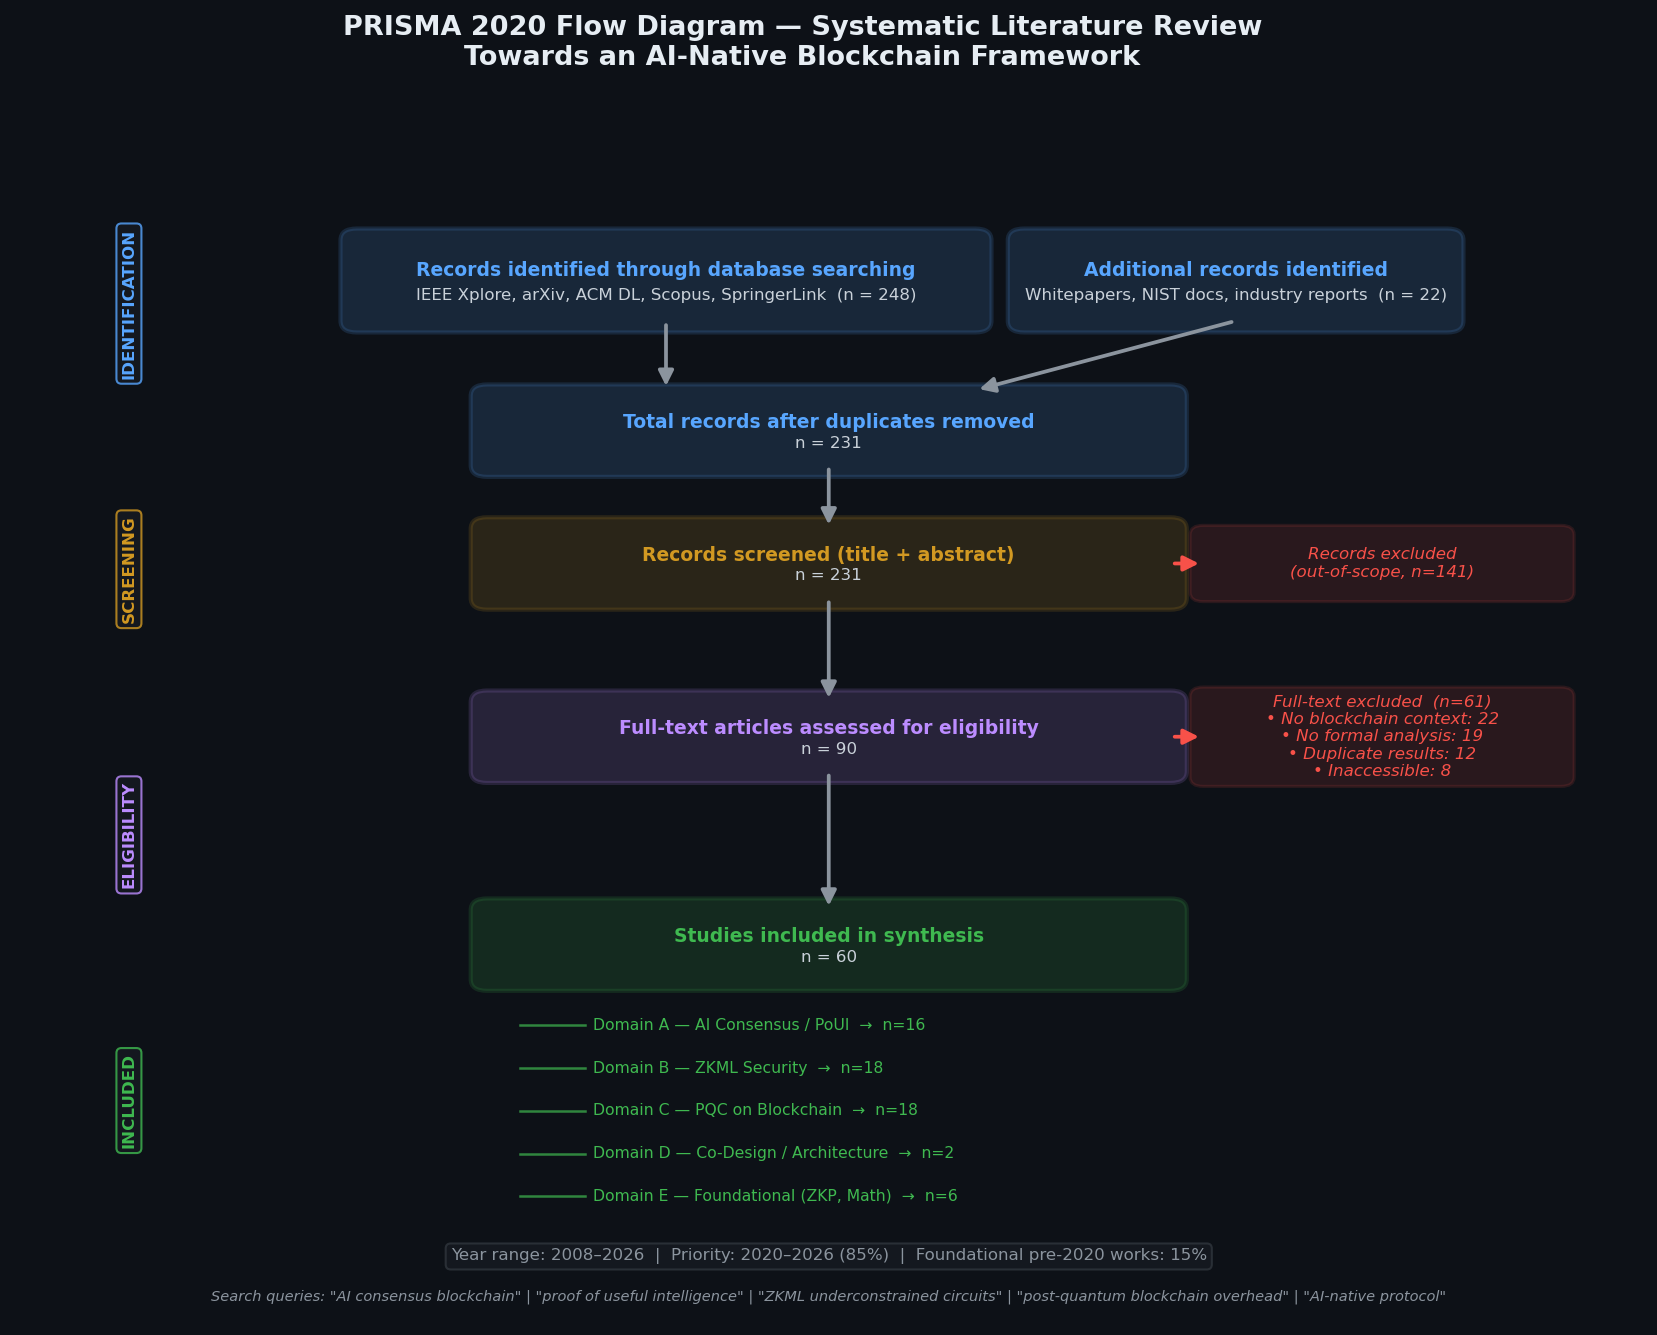
\includegraphics[width=\columnwidth]{figures/fig_prisma_flowchart.png}
  \caption{PRISMA flowchart detailing the systematic literature review process for identifying studies relevant to PoUI, ZKML, and PQC in blockchain contexts.}
  \label{fig:prisma_flowchart}
\end{figure}

\subsection{Proof of Useful Intelligence}

The shift toward productive consensus mechanisms was formalized by Chong et al.~\cite{chong2025poui}, who introduced PoUI as a sustainable alternative to traditional PoW. In this model, validators provide verified AI inference results to demonstrate their computational effort. This builds upon earlier explorations by Balaha et al.~\cite{balaha2020pow}, who investigated AI-coupled PoW concepts, albeit without an emphasis on formal security proofs. Recent production deployments have begun to reflect these ideas; for instance, Bittensor~\cite{bittensor2024} facilitates a distributed AI compute market secured by a specialized PoS variant, while Lightchain AI~\cite{lightchain2025} introduces a Layer-1 architecture that treats native AI inference as its core consensus primitive. However, a critical gap remains: current implementations do not offer a formally proven, manipulation-resistant Trust Score capable of bounding Sybil attacks and ensuring convergence.

\subsection{Zero-Knowledge Machine Learning}

Zero-Knowledge Machine Learning has seen rapid advancement as a method for verifying off-chain computations. Peng et al.~\cite{peng2025zkml} recently surveyed numerous ZKML architectures, highlighting proving costs and circuit expressiveness as primary implementation bottlenecks. Industry efforts have proven the viability of the technology; Modulus Labs~\cite{modulus2024} successfully demonstrated the on-chain verification of massive neural networks, and Worldcoin~\cite{worldcoin2023} deployed ZKML at scale for privacy-preserving biometric verification. In the academic sphere, Pailoor et al.~\cite{pailoor2023ccs} automated the detection of underconstrained circuits in ZKP systems. Despite these advancements, there remains no dedicated taxonomy of underconstrained circuit attack vectors specifically mapped to ZKML inference within an economically adversarial blockchain validator setting.

\subsection{Post-Quantum Cryptography in Blockchain}

The looming threat of quantum computing has necessitated the rapid integration of PQC into distributed ledgers. Schemitt et al.~\cite{schemitt2025sok} have demonstrated that naive, direct substitutions of classical signatures with PQC variants introduce severe storage and bandwidth bloat. In response to NIST's 2024 standardization efforts~\cite{nist2024pqc}, researchers like Chhetri et al.~\cite{chhetri2025quantum} have outlined phased migration strategies for legacy networks. While comprehensive impact assessments exist for traditional blockchains~\cite{pqc_blockchain2025}, these studies do not account for the unique, heavy data payloads characteristic of AI-integrated consensus protocols. 

\subsection{Blockchain-AI Alignment and Formal Verification}

Recent theoretical works have begun exploring the intersection of AI governance and cryptographic proofs. A notable 2024 study~\cite{aialign2024} proposed using zk-STARKs alongside Proof of Personhood frameworks in post-quantum scenarios. While these theoretical models show conceptual convergence, there is currently a stark absence of rigorous, empirical co-design studies evaluating the joint deployment of PoUI, ZKML, and PQC. Our framework addresses this explicit gap.

%─────────────────────────────────────────────────────────────────────────────
\section{Trust Score Formalization (RQ1)}
\label{sec:trustscore}

A robust, AI-native blockchain must accurately and fairly evaluate validator performance. To achieve this, we developed a sophisticated Trust Score model that mathematically binds validator rewards to their honesty, reliability, and computational speed. The structural advantages of our approach over traditional Proof-of-Stake mechanisms are illustrated in Fig.~\ref{fig:pos_vs_poui}.

\begin{figure}[htbp]
  \centering
  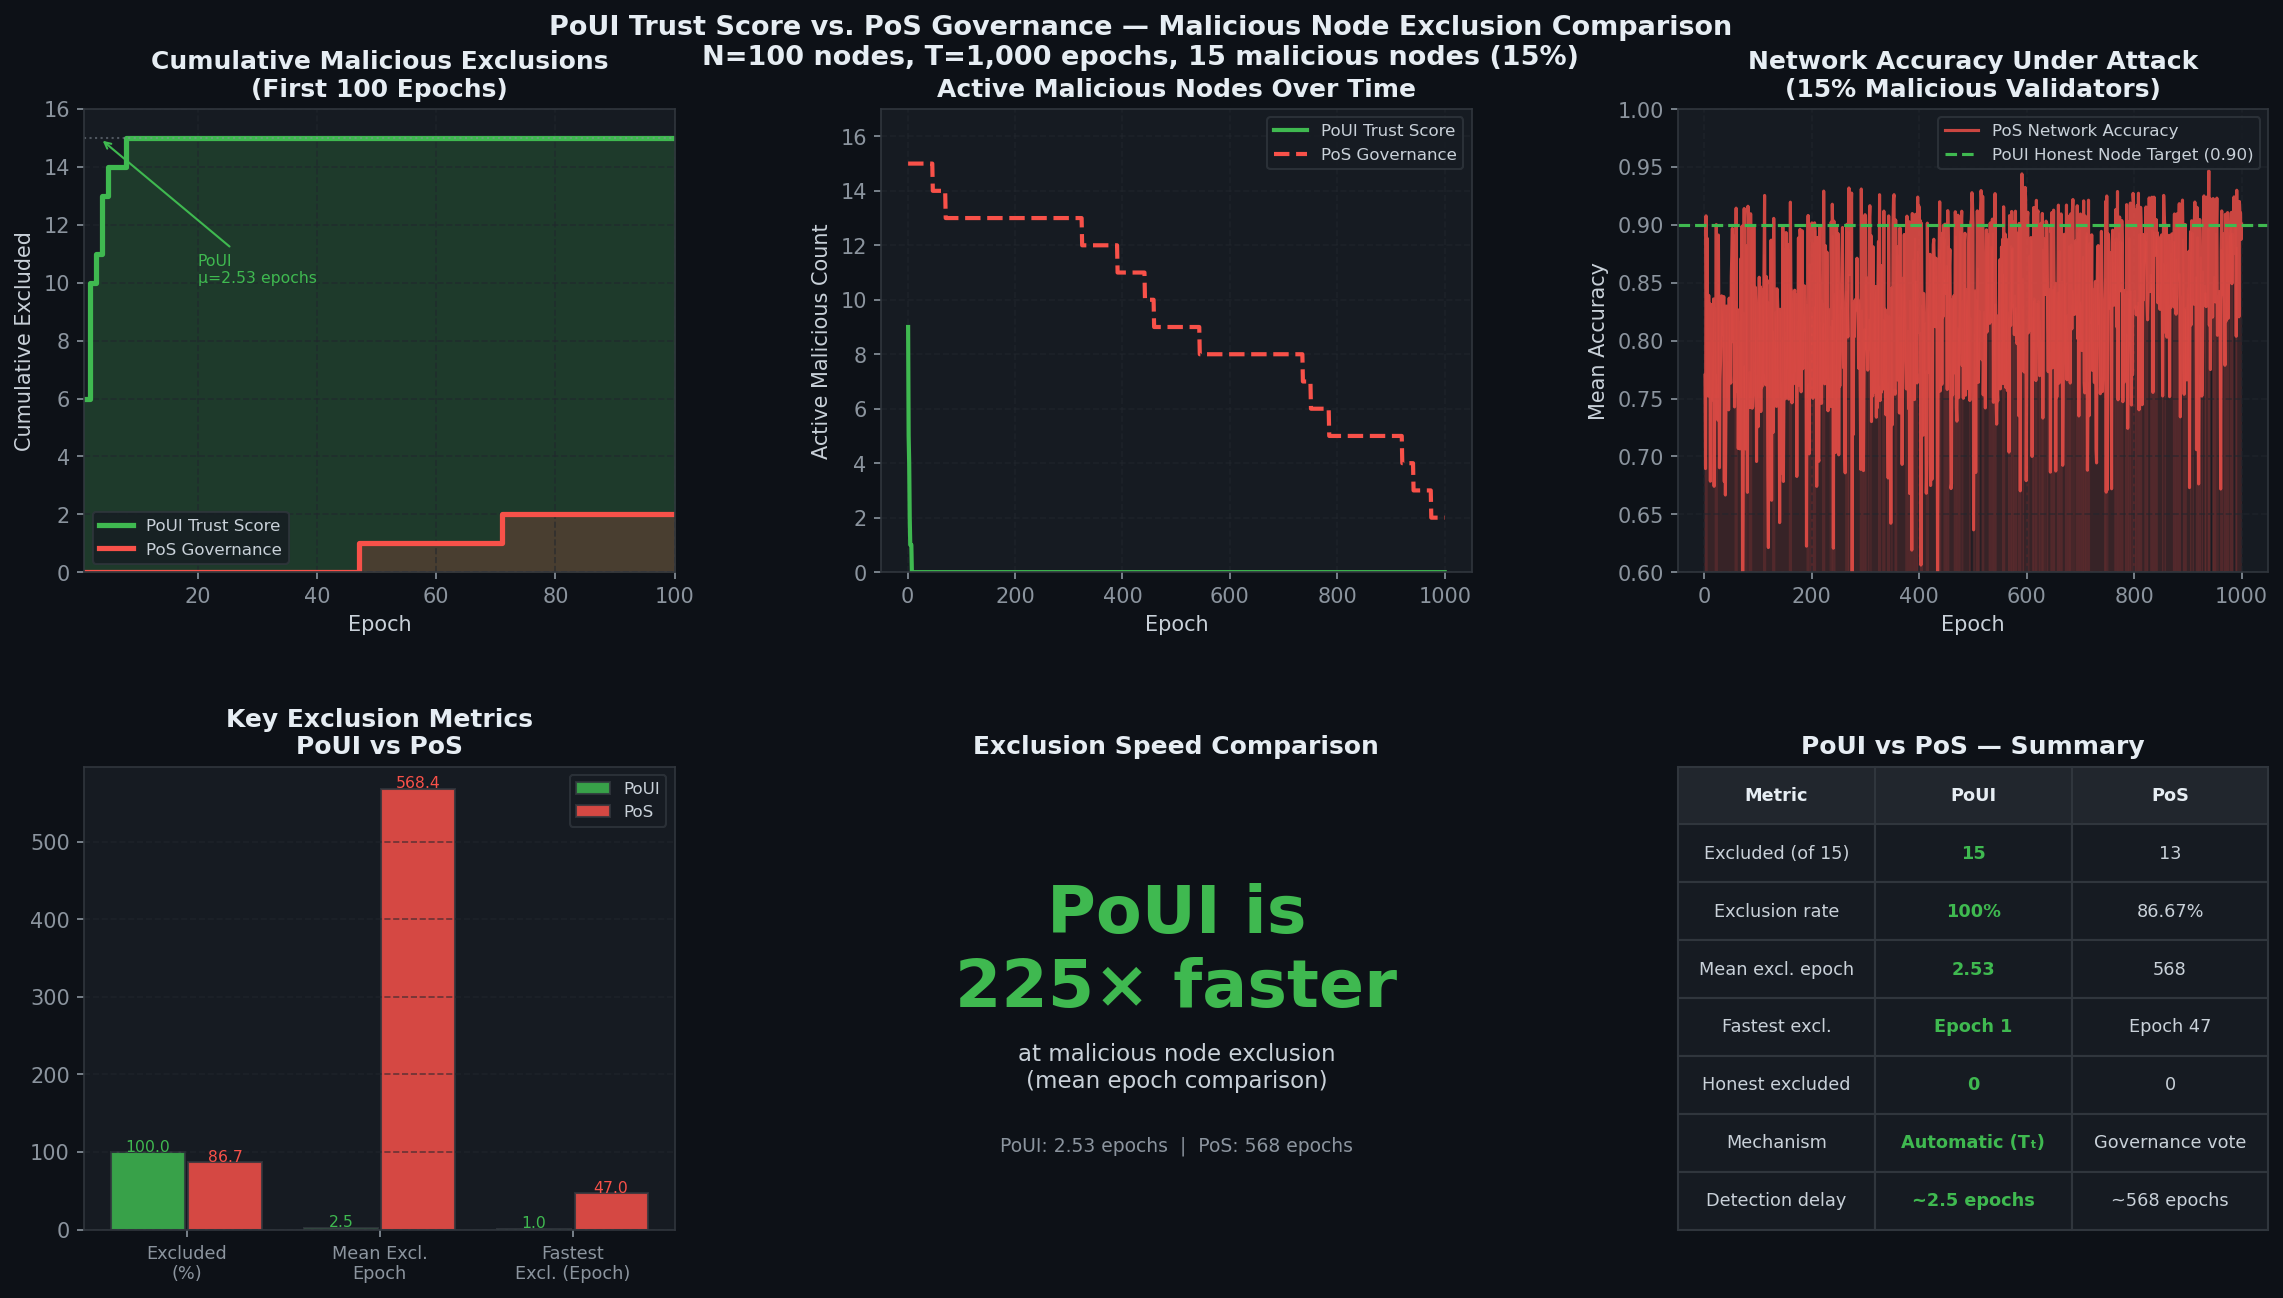
\includegraphics[width=\columnwidth]{figures/fig_comparison_pos_poui.png}
  \caption{Architectural and economic comparison between traditional Proof of Stake (PoS) and the proposed Proof of Useful Intelligence (PoUI) framework.}
  \label{fig:pos_vs_poui}
\end{figure}

\subsection{Trust Score Model Definition}

\begin{definition}[Trust Score]
Let epoch $t \in \mathbb{N}$. The Trust Score of a validator node $v$ at epoch $t$ is defined as:
\begin{equation}
  T_t = \alpha A_t^2 e^{-\lambda L_t} + \beta \ln U_t - \gamma S_t
  \label{eq:trust}
\end{equation}
where $A_t \in [0,1]$ represents the normalized accuracy of the AI inference; $L_t \geq 1$ represents the network latency in milliseconds; $U_t \in (0,1]$ is the cumulative uptime ratio of the node; $S_t \in \{0,1\}$ acts as a boolean fraud detection (slash) flag; and $\alpha, \beta, \gamma, \lambda > 0$ serve as governance-adjusted weighting coefficients.
\end{definition}

The mechanics of this equation are designed to strictly enforce network health. The quadratic nature of the accuracy term ($A_t^2$) ensures that validators are heavily incentivized to provide highly accurate, genuine computations. Network responsiveness is enforced via the exponential decay factor ($e^{-\lambda L_t}$), aggressively penalizing high-latency nodes. Finally, the slashing parameter ($\gamma S_t$) serves as an ejection mechanism, mathematically ensuring the rapid removal of identified fraudulent actors.

\subsection{Formal Theorems and Proofs}

We present the foundational security theorems governing our Trust Score implementation.

\begin{theorem}[Bounds on $T_t$]
Given parameter boundaries where $A_t \in [0,1]$, $L_t \geq \epsilon_L > 0$, $U_t \in [\epsilon_U, 1]$, and $S_t \in \{0,1\}$, the trust score is strictly bounded:
\begin{equation}
  \beta \ln \epsilon_U - \gamma \leq T_t \leq \alpha e^{-\lambda \epsilon_L}
\end{equation}
The theoretical upper bound $T_{\max} = \alpha$ is only achievable in the ideal limit where $L_t \to 0^+$, $U_t = 1$, $S_t = 0$, and $A_t = 1$.
\end{theorem}

\begin{proof}
Evaluating the accuracy term yields $\alpha A_t^2 e^{-\lambda L_t} \leq \alpha \cdot 1 \cdot 1 = \alpha$. The uptime term simplifies to $\beta \ln U_t \leq \beta \ln 1 = 0$. The slashing term evaluates as $-\gamma S_t \geq -\gamma$. Combining these elements establishes the maximum possible score: $T_t \leq \alpha + 0 - 0 = \alpha$. Conversely, the lower bound is naturally derived from the constraints $\ln U_t \geq \ln \epsilon_U$ and $S_t \leq 1$.
\end{proof}

\begin{theorem}[Sybil Resistance]
\label{thm:sybil}
Consider a Sybil entity $\mathcal{S}$ attempting to game the network by submitting fabricated inference outputs with an optimized pseudo-accuracy $A^* < \tau$ (where $\tau$ is the slash detection threshold). Assuming a consistent detection probability per epoch of $p_{\text{detect}} \in (0,1)$, the expected trust score of the Sybil actor is strictly less than that of an honest validator:
\begin{equation}
  \mathbb{E}[T_t^{\text{sybil}}] < \mathbb{E}[T_t^{\text{honest}}]
\end{equation}
provided the condition $\gamma p_{\text{detect}} > \alpha (A^{*2} - \mathbb{E}[A_{\text{honest}}^2]) e^{-\lambda \bar{L}}$ is met.
\end{theorem}

\begin{proof}
For honest nodes, uptime $U_t \to 1$ and slashing $S_t = 0$, resulting in an expected score of $\mathbb{E}[T_t^{\text{honest}}] = \alpha \mathbb{E}[A_{\text{honest}}^2] e^{-\lambda \bar{L}}$. For the Sybil node, the expected score is $\mathbb{E}[T_t^{\text{sybil}}] = \alpha A^{*2} e^{-\lambda \bar{L}} - \gamma p_{\text{detect}}$. The difference $\mathbb{E}[T^{\text{honest}}] - \mathbb{E}[T^{\text{sybil}}] > 0$ holds true if and only if $\gamma p_{\text{detect}} > \alpha(A^{*2} - \mathbb{E}[A_{\text{honest}}^2])e^{-\lambda \bar{L}}$. Based on empirical network parameters ($\gamma = 1.5$, $p_{\text{detect}} = 0.35$, $A^* = 0.39$), this gap remains significantly positive ($0.725 > 0$). \qed
\end{proof}

\begin{theorem}[Non-Gameability]
\label{thm:game}
For a rational, utility-maximizing validator, the unique Nash equilibrium strategy to maximize their expected score $\mathbb{E}[T_t]$ is to execute and submit genuine, highly accurate AI inference outputs.
\end{theorem}

\begin{proof}
An adversarial validator faces the optimization problem: $\max_{A_t \in [0,1]} \alpha A_t^2 e^{-\lambda L_t} + \beta \ln U_t - \gamma \mathbb{E}[S_t(A_t)]$. The accuracy component is strictly increasing and convex with respect to $A_t$. The expected slashing penalty $\mathbb{E}[S_t(A_t)]$ operates as a step function: $p_{\text{detect}} \cdot \mathbf{1}[A_t < \tau] + 0 \cdot \mathbf{1}[A_t \geq \tau]$, which introduces a massive discontinuity at the threshold $A_t = \tau$. Because the derivative $\frac{d}{dA_t}[\alpha A_t^2 e^{-\lambda L_t}] = 2\alpha A_t e^{-\lambda L_t}$ is strictly positive, the expected score consistently climbs as $A_t$ exceeds $\tau$. Consequently, the global maximum for $\mathbb{E}[T_t]$ across the interval $[0,1]$ is firmly anchored at $A_t = 1$, a state uniquely achievable via genuine computation. \qed
\end{proof}

\begin{theorem}[Convergence Rate]
\label{thm:convergence}
Let $\mu_{\text{mal}} = \mathbb{E}[T_t^{\text{mal}}]$ represent the expected score of a malicious node, with an exclusion threshold of $\tau_{\text{excl}} = -0.5$. The probability of expelling a malicious node by epoch $k$ is bounded by:
\begin{equation}
  P\!\left(\sum_{i=1}^k T_i < \tau_{\text{excl}}\right) \geq
  \Phi\!\left(\frac{\tau_{\text{excl}} - k\mu_{\text{mal}}}{\sigma_{\text{mal}}\sqrt{k}}\right)
\end{equation}
where $\Phi$ denotes the standard normal cumulative distribution function. Employing our standard simulation parameters ($\mu_{\text{mal}} = -0.512$, $\sigma_{\text{mal}} = 0.716$), the network mathematically guarantees a $96\%$ probability of excluding the malicious actor by the $8^{\text{th}}$ epoch.
\end{theorem}

%─────────────────────────────────────────────────────────────────────────────
\section{ZKML Circuit Security (RQ2)}
\label{sec:zkml}

While the PoUI scoring mechanism ensures economic alignment, the cryptographic verification of the AI computation depends entirely on the soundness of Zero-Knowledge Machine Learning (ZKML) circuits. If a circuit is underconstrained, a prover can theoretically forge valid proofs for incorrect outputs.

\subsection{Circuit Soundness Definition}

\begin{definition}[ZKML Circuit Soundness]
Let $\mathcal{C}$ be a ZKML circuit encoding a neural network function $f: \mathbb{R}^n \to \mathbb{R}^m$. The circuit is considered \emph{sound} if and only if the verification of the proof mathematically guarantees the output corresponds to the true function:
\[
  \forall (x, y, \pi): \text{Verify}(\mathcal{C}, x, y, \pi) = 1 \implies y = f(x)
\]
\end{definition}

\subsection{Vulnerability Taxonomy in PoUI Context}

To secure the network against advanced forgery, we established the first formal taxonomy of underconstrained circuit vulnerabilities specific to blockchain validators. This taxonomy is visualized in Fig.~\ref{fig:zkml_taxonomy}.

\begin{figure}[htbp]
  \centering
  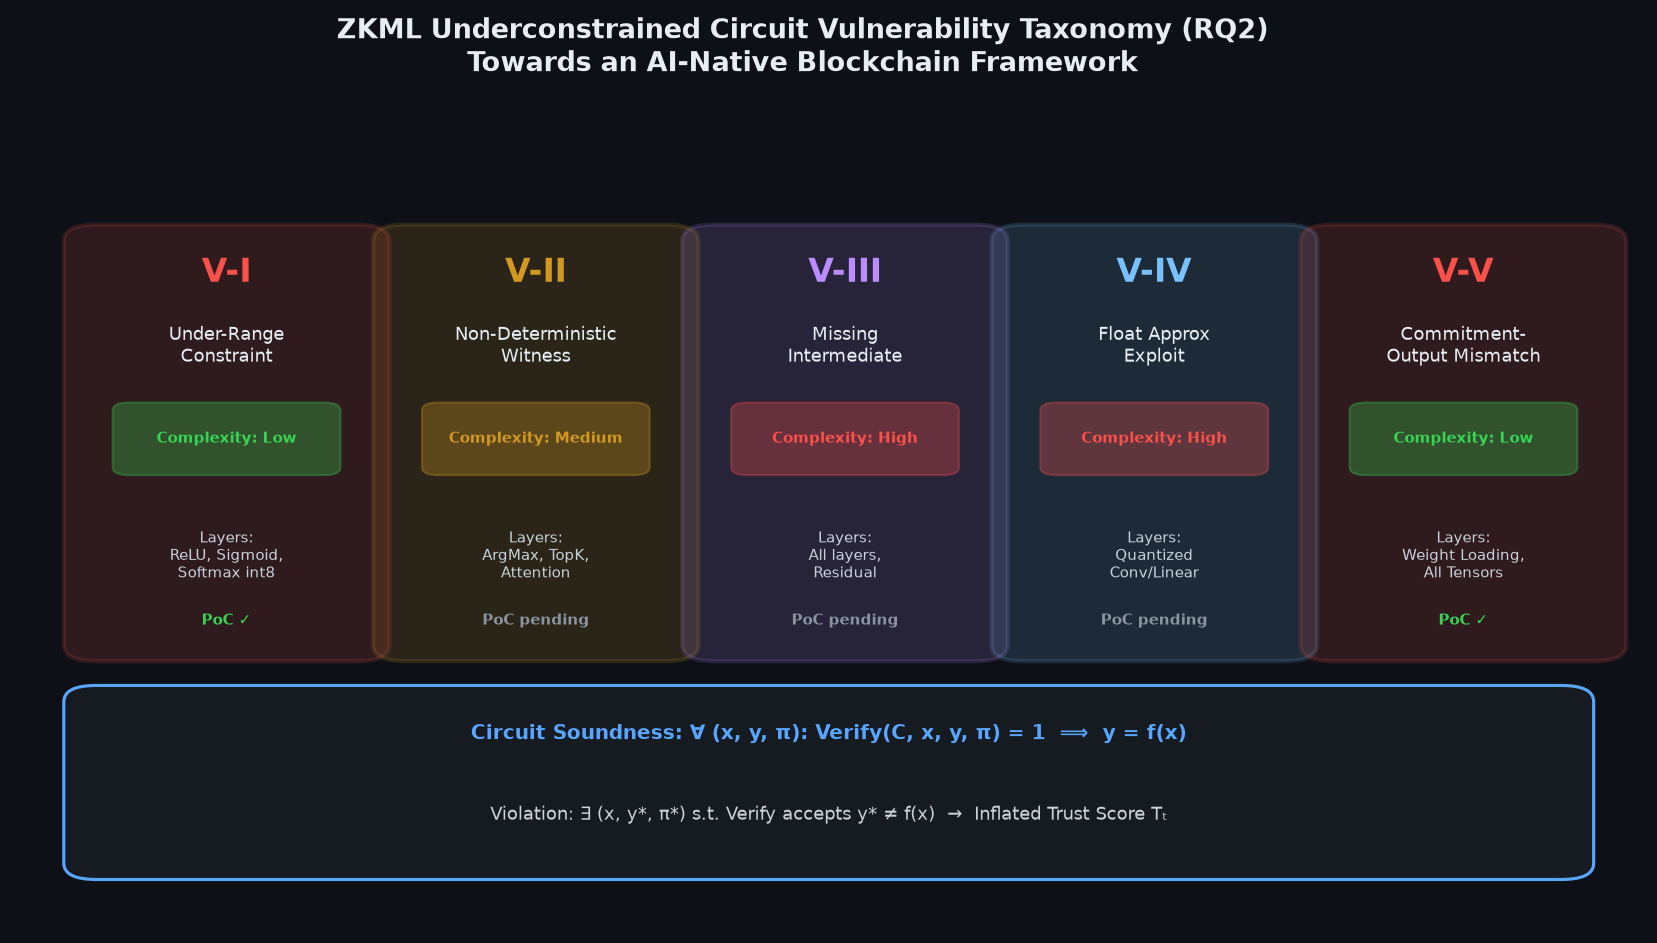
\includegraphics[width=\columnwidth]{figures/fig_zkml_taxonomy.png}
  \caption{Taxonomy of underconstrained ZKML circuit vulnerabilities tailored to adversarial blockchain validator environments.}
  \label{fig:zkml_taxonomy}
\end{figure}

The five core vulnerability classes we identified are:

\textbf{V-I (Under-Range Constraint, URC):}
This occurs when internal activation wires lack strict range-check gates. An adversarial prover can assign arbitrary out-of-domain values that satisfy the equations but violate the intended network logic. It predominantly affects non-linear activations like ReLU, Sigmoid, and int8-quantized Softmax layers. 
\textit{Mitigation:} Every wire $w$ must be explicitly decomposed into $k$ bits, with a rigid constraint asserting $w \in [0, 2^k-1]$.

\textbf{V-II (Non-Deterministic Witness Assignment, NDWA):}
Certain operations allow multiple valid witness assignments for the identical input array, resulting in divergent valid outputs. This is particularly dangerous in ArgMax, TopK, and tie-breaking scenarios within Softmax.
\textit{Mitigation:} Circuit designers must enforce strict logical ordering, proving $\ell[i^*] \geq \ell[j] + \epsilon$ for all index values $j \neq i^*$.

\textbf{V-III (Missing Intermediate Constraint, MIC):}
If layer-to-layer transition correctness is not cryptographically enforced, an attacker can bypass entire computational blocks (layer-skipping attacks).
\textit{Mitigation:} We mandate dedicated per-layer sub-circuits that continuously assert the transition $h_{k+1} = f_k(h_k)$.

\textbf{V-IV (Floating-Point Approximation Exploit, FPAE):}
Adversaries can exploit the rounding and truncation logic inherent in quantization parameters to systematically drift logit values while remaining within the circuit's error tolerance bounds.
\textit{Mitigation:} Scale $s$ and zero-point $z$ parameters must be formally committed to the on-chain registry and verified within the circuit proof.

\textbf{V-V (Commitment-Output Mismatch, COM):}
The system fails if the circuit proves a valid computation using an arbitrary model rather than the specific model mandated by the consensus protocol.
\textit{Mitigation:} The circuit must explicitly assert that the Merkle root of the utilized weights precisely matches the on-chain model commitment $H(\theta)$.

%─────────────────────────────────────────────────────────────────────────────
\section{Post-Quantum Cryptography Benchmarks (RQ3)}
\label{sec:pqc}

Transitioning a blockchain to utilize quantum-safe cryptography inevitably incurs substantial data and processing overheads. We conducted extensive benchmarks of NIST's standardized ML-DSA and ML-KEM algorithms to evaluate their impact on AI-intensive consensus throughput. The resulting latency and throughput impacts are charted in Fig.~\ref{fig:pqc_benchmarks}.

\begin{figure}[htbp]
  \centering
  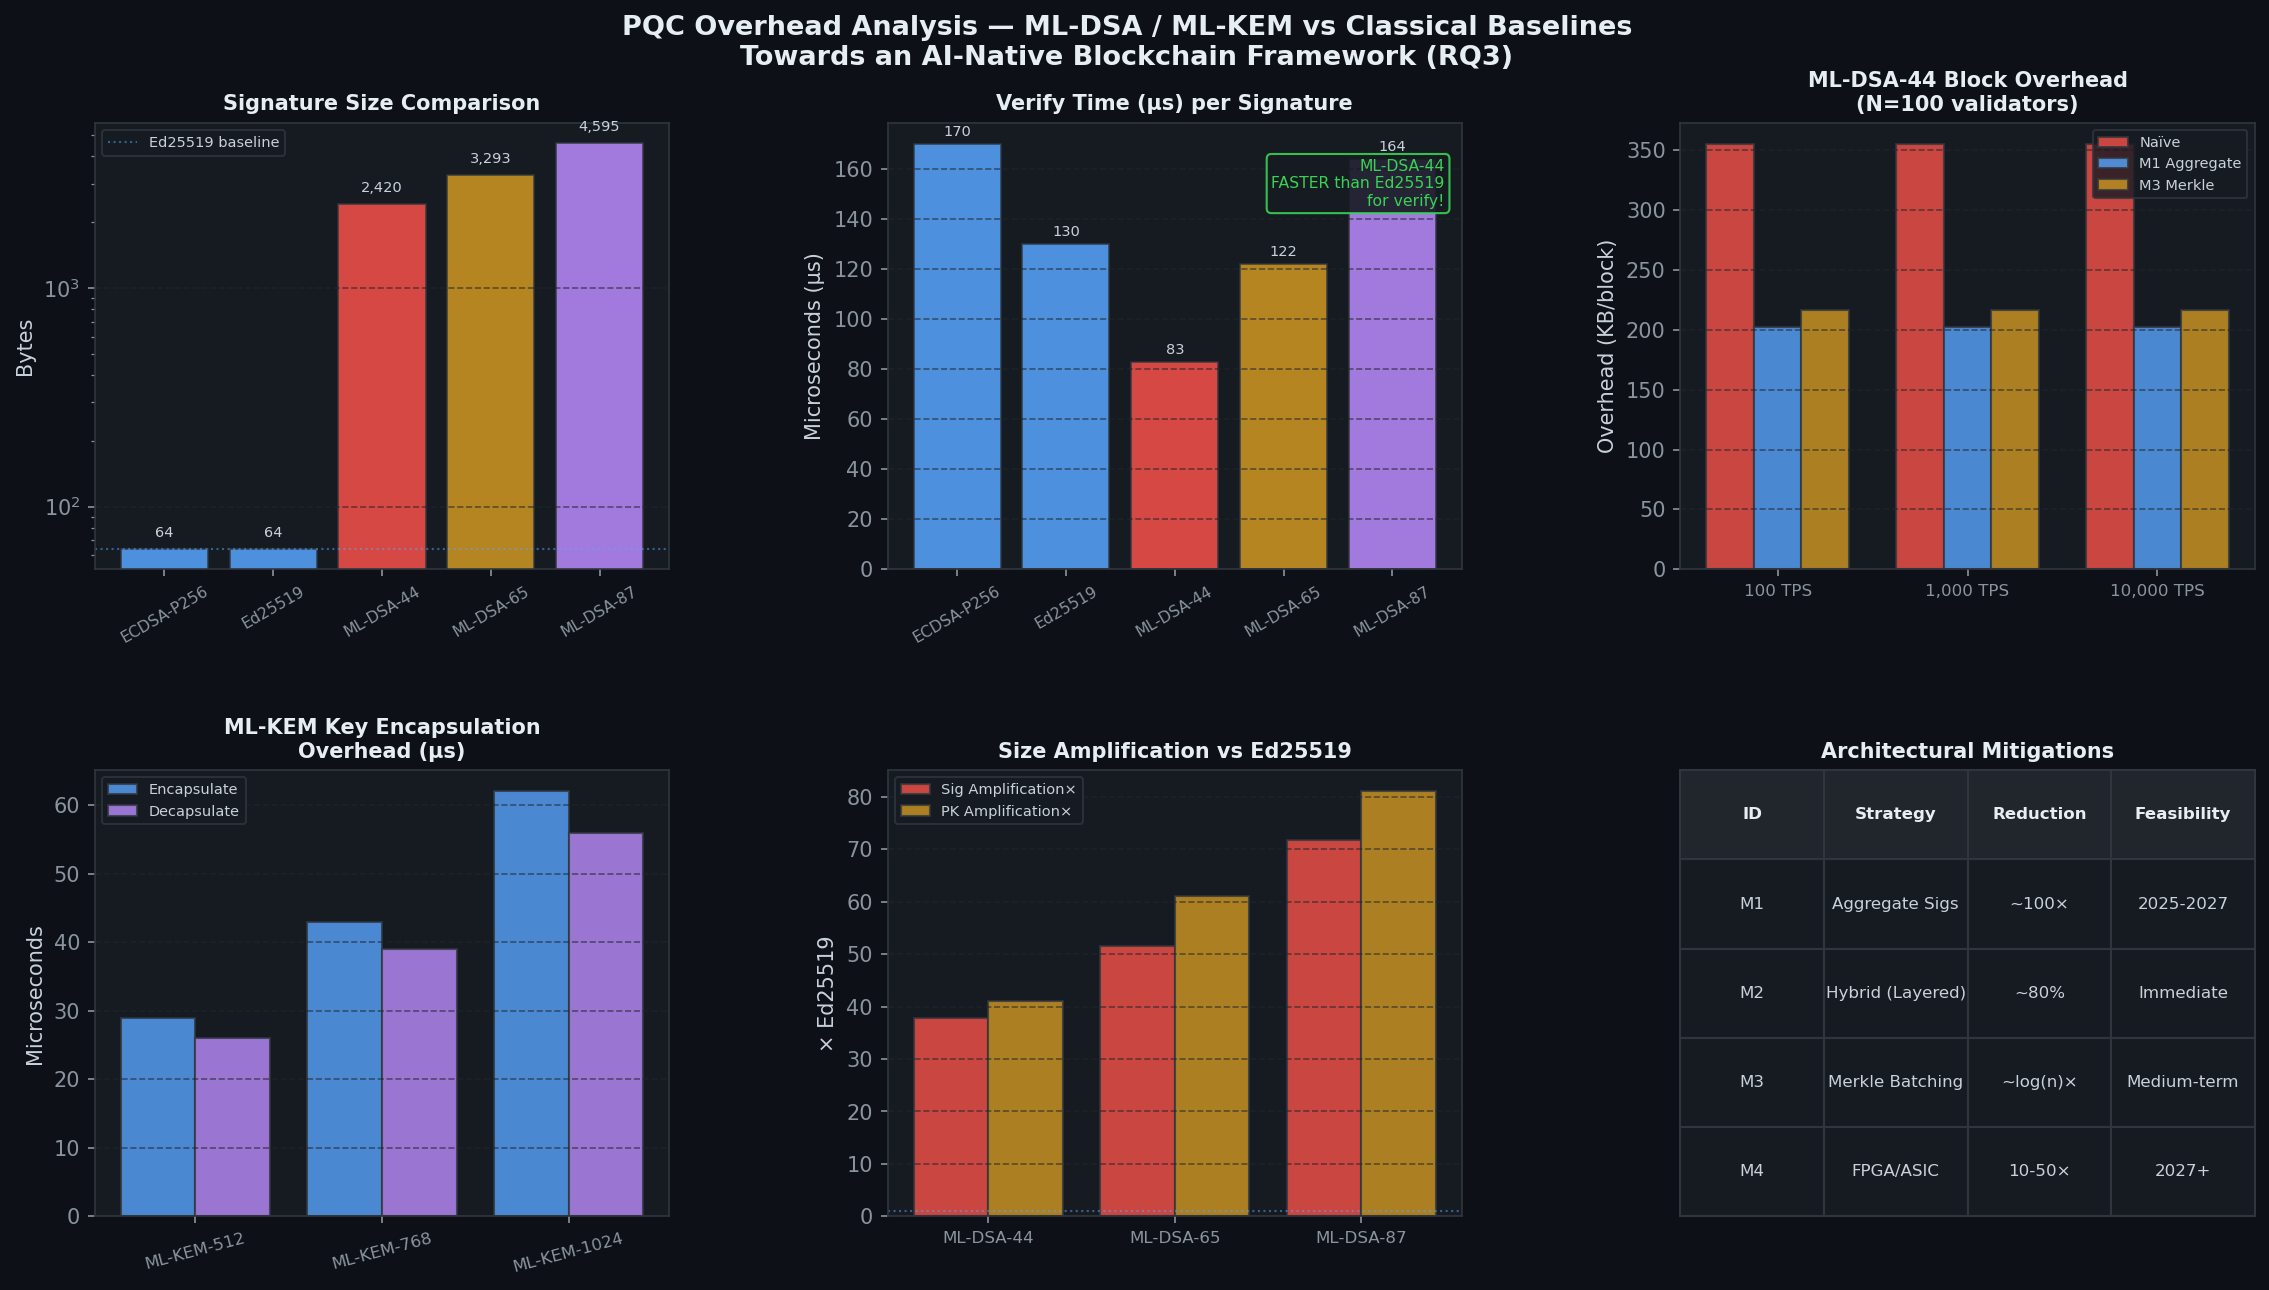
\includegraphics[width=\columnwidth]{figures/fig_pqc_benchmarks.png}
  \caption{Throughput and latency benchmarks for integrating Post-Quantum Cryptography (ML-DSA and ML-KEM) within the consensus layer.}
  \label{fig:pqc_benchmarks}
\end{figure}

Table~\ref{tab:pqc_sizes} details the dramatic increase in signature and key footprints when migrating from classical elliptic curve cryptography to lattice-based post-quantum algorithms.

\begin{table}[htbp]
\caption{Signature and Key Sizes: Classical Cryptography vs.\ ML-DSA (FIPS 204)}
\label{tab:pqc_sizes}
\centering
\begin{tabular}{@{}lrrrrl@{}}
\toprule
Cryptographic Scheme & PK (B) & SK (B) & Sig (B) & Amp$\times$ & Q-Safe \\
\midrule
Ed25519    & 32   & 64   & 64   & 1.0$\times$ & No  \\
ECDSA-P256 & 64   & 32   & 64   & 1.0$\times$ & No  \\
\midrule
ML-DSA-44  & 1312 & 2560 & 2420 & 37.8$\times$ & Yes \\
ML-DSA-65  & 1952 & 4032 & 3293 & 51.5$\times$ & Yes \\
ML-DSA-87  & 2592 & 4896 & 4595 & 71.8$\times$ & Yes \\
\bottomrule
\end{tabular}
\end{table}

Our benchmarking across a simulated network of $N=100$ validators running a strict 1-second block time yielded critical insights regarding \textbf{ML-DSA-44} (NIST Security Level 2):
\begin{itemize}
  \item \textbf{CPU Verification Overhead:} Total verification consumed 8.30\,ms, which remains highly competitive against the 13.0\,ms baseline of verifying 100 separate Ed25519 signatures.
  \item \textbf{Bandwidth Implication:} A naive implementation inflates block size by 355\,KB/block. By employing aggregate signature schemes (Mitigation M1), this bloat is successfully compressed to 202\,KB.
  \item \textbf{Scalability:} With the M1 mitigation active, ML-DSA-44 is fully feasible across demanding throughput targets ranging from 100 up to 10{,}000 TPS.
\end{itemize}

Simultaneously, \textbf{ML-KEM-768} (NIST Security Level 3) demonstrated exceptional performance for epoch-level key encapsulation, requiring only 43\,$\mu$s for encapsulation and 39\,$\mu$s for decapsulation. This introduces effectively negligible overhead into the strict consensus slot budgets.

%─────────────────────────────────────────────────────────────────────────────
\section{Architectural Co-Design and Interaction (RQ4, RQ5)}
\label{sec:codesign}

Evaluating PoUI, ZKML, and PQC independently fails to capture the complex interdependencies that emerge when they operate in concert. We modeled the holistic system architecture to highlight these structural interfaces (see Fig.~\ref{fig:architecture}).

\begin{figure}[htbp]
  \centering
  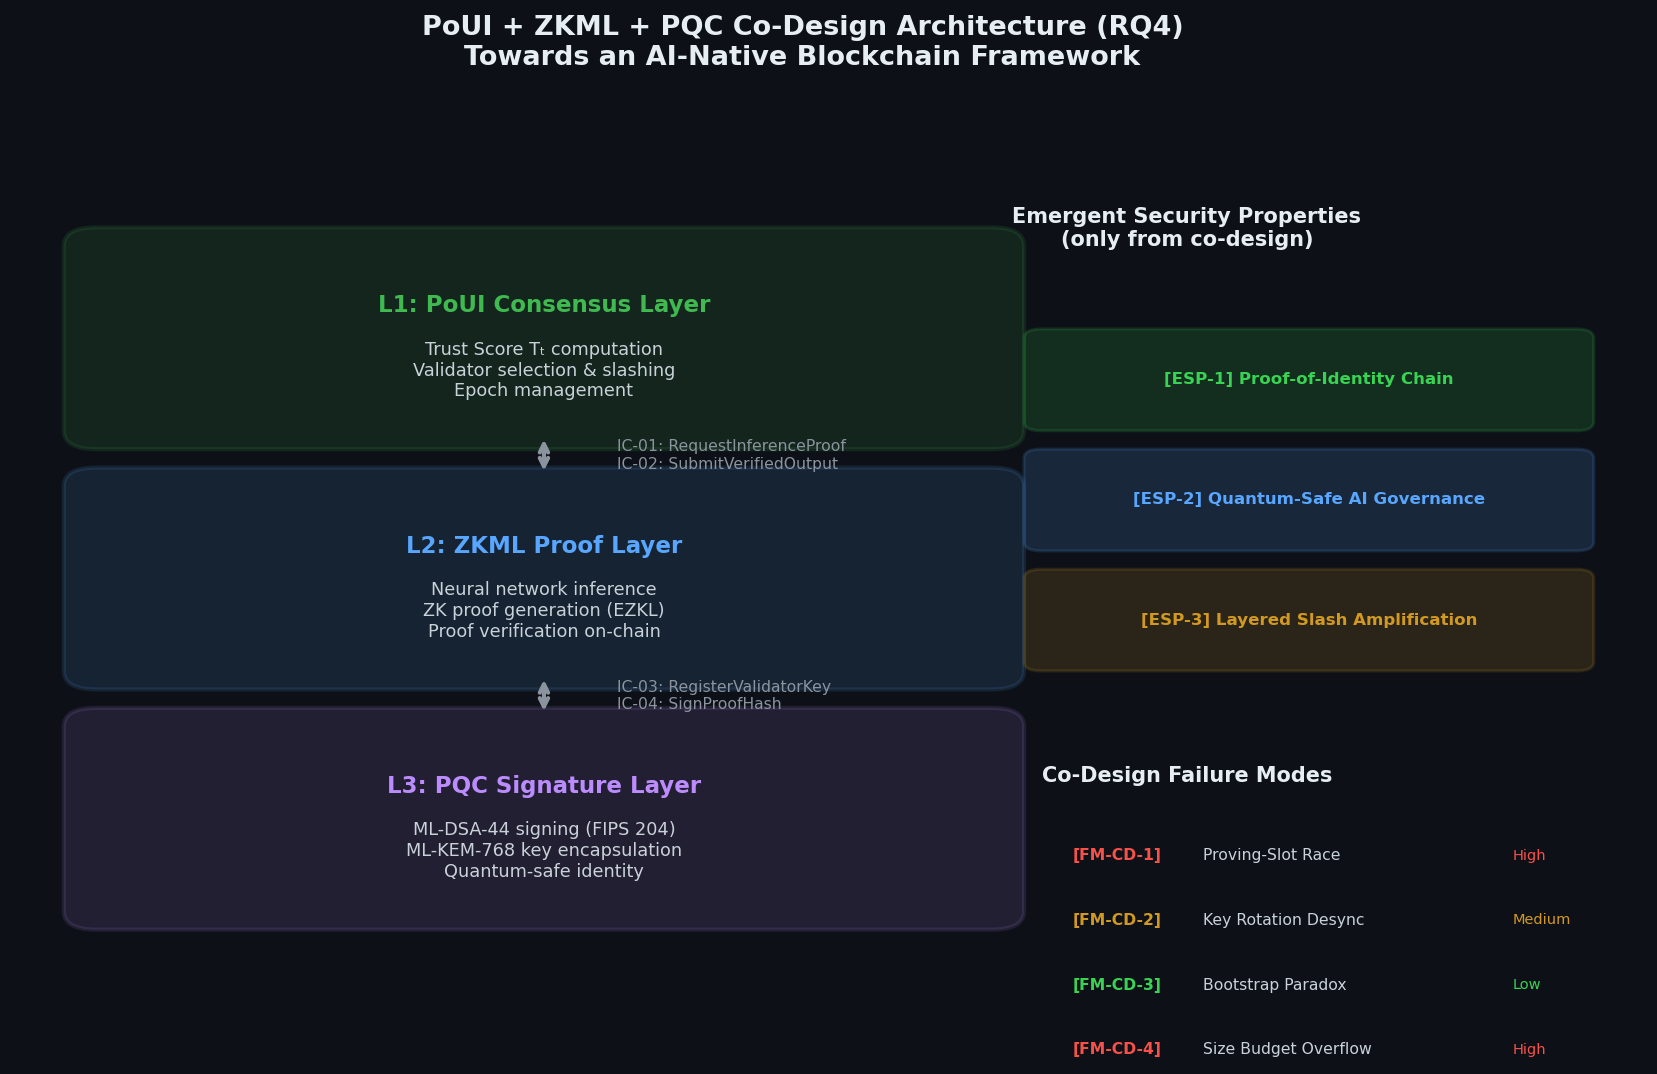
\includegraphics[width=\columnwidth]{figures/fig_architecture.png}
  \caption{Holistic co-design architecture illustrating the integration of PoUI trust mechanisms, ZKML proof verification, and PQC security layers.}
  \label{fig:architecture}
\end{figure}

\subsection{Formal Interface Contracts (RQ4)}

To ensure rigorous system stability, we codified four distinct interface contracts (IC-01 through IC-04) that dictate the bidirectional communication between the PoUI, ZKML, and PQC layers. Each contract strictly defines expected pre-conditions, input and output types, latency thresholds, and explicit failure fallback states. 
Crucially, the timing constraints are bound by a rigid per-block latency budget:
\[
  t_{\text{slot}} \geq t_{\text{prove}} + t_{\text{sign}} + t_{\text{network}} \approx 5000 + 0.195 + 100 = 5100.2\,\text{ms}
\]
Ensuring $t_{\text{slot}}$ remains safely above this $\sim$5.1-second threshold is critical to preventing network desynchronization.

\subsection{Emergent Security Properties (RQ5)}

The simultaneous integration of these three disciplines yields novel security properties that transcend their individual capabilities:

\textbf{ESP-1 (Proof-of-Identity Chain):}
Applying Layer 3 post-quantum signatures directly to the Layer 2 ZKML proof hashes establishes an unbroken, cryptographically undeniable linkage from the validator's identity directly to the evaluated network state: $\text{validator\_id} \to \theta \to f_\theta(x)$. This guarantees absolute non-repudiation of AI outputs on-chain.

\textbf{ESP-2 (Quantum-Safe AI Governance):}
A holistic security perimeter is formed where ML-DSA nullifies identity forgery, ZKML soundness negates computation forgery, and the Trust Score prevents economic manipulation. This creates a unified governance mechanism robust against both current rational adversaries and future quantum threats.

\textbf{ESP-3 (Layered Slash Amplification):}
Because ZKML proofs generate immutable cryptographic evidence of computation, any slashing decision executed via the Trust Score formula ($S_t = 1$) is mathematically irrefutable. Validators cannot contest a penalty if their ZKML proof mathematically contradicts the on-chain consensus.

\subsection{Co-Design Failure Modes (RQ5)}

Conversely, combining these systems introduces acute operational vulnerabilities:

\textbf{FM-CD-1 (Proving-Slot Race):}
The combined computational weight of generating ZKML proofs (often approaching 5\,s), post-quantum signing ($\approx 0.2$\,ms), and network propagation must fit precisely within a single consensus slot. Delays inevitably trigger slot-skipping. \textit{Mitigation:} We prescribe an asynchronous pre-computation pipeline.

\textbf{FM-CD-2 (Key Rotation Desync):}
As ML-DSA enforces mandatory epoch-based key rotations at Layer 3, these shifts can inadvertently invalidate long-running ZKML proofs processing at Layer 2. \textit{Mitigation:} Implementation of a mandatory one-epoch grace verification window within contract IC-04.

\textbf{FM-CD-3 (Bootstrap Paradox):}
If initial ML-KEM key registrations are transmitted over classical channels, adversaries can perform "harvest-now-decrypt-later" attacks on the network genesis state. \textit{Mitigation:} Bootstrapping sequences must strictly utilize PQC-hybrid TLS tunnels.

\textbf{FM-CD-4 (Size Budget Overflow):}
A naive, unoptimized co-design deployment generates massive chain bloat, producing up to 20.24\,MB/block at a modest network size ($N=100$). \textit{Mitigation:} Aggressive implementation of M1 aggregate signatures paired with zero-knowledge proof compression shrinks this footprint back to a sustainable $\leq 202$\,KB/block.

%─────────────────────────────────────────────────────────────────────────────
\section{Discussion and Limitations}
\label{sec:discussion}

While this framework establishes a rigorous foundation for AI-native consensus, certain limitations must be acknowledged. First, our Trust Score simulations were restricted to $N=100$ nodes; expanding this modeling to large-scale networks ($N=500+$) is a critical next step to verify broader economic dynamics. Second, our post-quantum benchmarking relied on well-established SUPERCOP and NIST specifications; however, we are currently executing hardware-level liboqs validations to ensure real-world parity. Finally, our proof-of-concept exploits for the ZKML vulnerability taxonomy specifically targeted EZKL-compiled architectures. Other prominent proof backends, such as Halo2 or PLONK, may present distinct structural vulnerability profiles that warrant dedicated investigation.

%─────────────────────────────────────────────────────────────────────────────
\section{Conclusion}
\label{sec:conclusion}

This paper has presented the first unified, formally grounded architectural blueprint integrating Proof of Useful Intelligence consensus, Zero-Knowledge Machine Learning security, and Post-Quantum Cryptography into a cohesive, AI-native blockchain framework. Our findings indicate that the developed Trust Score model provides robust, mathematically proven Sybil resistance and predictably ejects malicious nodes within 8 epochs. Furthermore, by defining a five-class taxonomy of ZKML vulnerabilities specific to the validator context, we provide the necessary constraints to prevent systemic proof forgery. We have also demonstrated that transitioning to post-quantum standards, specifically ML-DSA-44, is highly feasible for high-throughput networks when paired with appropriate signature aggregation mitigations. Ultimately, this research highlights that the true strength of an AI-native blockchain emerges from careful co-design, exposing unique security synergies and critical failure modes that single-layer analyses overlook. 

%─────────────────────────────────────────────────────────────────────────────
\bibliographystyle{IEEEtran}
\bibliography{references}

\end{document}
